\documentclass[12pt]{article}
\usepackage{amsthm,amssymb,amsfonts,amsmath,amstext,systeme}
\usepackage{graphicx,float}
\usepackage{tabularx}

\marginparwidth 0pt
\oddsidemargin -1.2 truecm
\evensidemargin  0pt 
\marginparsep 0pt
\topmargin -2.2truecm
\linespread{1}
\textheight 25.8 truecm
\textwidth 18.5 truecm
\newenvironment{remark}{\noindent{\bf Remark }}{\vspace{0mm}}
\newenvironment{remarks}{\noindent{\bf Remarks }}{\vspace{0mm}}
\newenvironment{question}{\noindent{\bf Question }}{\vspace{0mm}}
\newenvironment{questions}{\noindent{\bf Questions }}{\vspace{0mm}}
\newenvironment{note}{\noindent{\bf Note }}{\vspace{0mm}}
\newenvironment{summary}{\noindent{\bf Summary }}{\vspace{0mm}}
\newenvironment{back}{\noindent{\bf Background}}{\vspace{0mm}}
\newenvironment{conclude}{\noindent{\bf Conclusion}}{\vspace{0mm}}
\newenvironment{concludes}{\noindent{\bf Conclusions}}{\vspace{0mm}}
\newenvironment{dill}{\noindent{\bf Description of Dill's model}}{\vspace{0mm}}
\newenvironment{maths}{\noindent{\bf Mathematics needed}}{\vspace{0mm}}
\newenvironment{inst}{\noindent{\bf Instructions}}{\vspace{0mm}}
\newenvironment{notes}{\noindent{\bf Notes }}{\vspace{0mm}}
\newenvironment{theorem}{\noindent{\bf Theorem }}{\vspace{0mm}}
\newenvironment{example}{\noindent{\bf Example }}{\vspace{0mm}}
\newenvironment{examples}{\noindent{\bf Examples }}{\vspace{0mm}}
\newenvironment{topics}{\noindent{\bf Topics}}{\vspace{0mm}}
\newenvironment{outcomes}{\noindent{\bf Expected Learning Outcomes}}{\vspace{0mm}}
\newenvironment{lemma}{\noindent{\bf Lemma }}{\vspace{0mm}}
\newenvironment{solution}{\noindent{\it Solution}}{\vspace{2mm}}
\newcommand{\ds}{\displaystyle}
\newcommand{\un}{\underline}
\newcommand{\bs}{\boldsymbol}

\begin{document}

\baselineskip 18 pt
\begin{center}
	{\large \bf HKDSE MATH CORE 2019 Past Paper I}\\
	\vspace{2 mm}

\end{center}
\vspace{0.05cm}

\begin{enumerate}
	\item \textbf{HKDSE MATH CORE 2019 Past Paper I Q1}\\
	Make $h$ the subject of the formula $9(h + 6k) = 7h + 8$. \\(3 marks)

	\item \textbf{HKDSE MATH CORE 2019 Past Paper I Q2}\\
	Simplify $\dfrac{3}{7x - 6} - \dfrac{2}{5x - 4}$. \\(3 marks)

	\item \textbf{HKDSE MATH CORE 2019 Past Paper I Q3}\\
	The length and the breadth of a rectangle are 24 cm and $(13 + r)$ cm respectively. If the length of a diagonal of the rectangle is $(17 - 3r)$ cm, find $r$. \\(3 marks)

	\item \textbf{HKDSE MATH CORE 2019 Past Paper I Q4}
	Factorize
	\begin{enumerate}
		\item[(a)] $4m^2 - 9$,
		\item[(b)] $2m^2n + 7mn - 15n$.
		\item[(c)] $4m^2 - 9 - 2m^2n - 7mn + 15n$.
	\end{enumerate}
	(4 marks)

	\item \textbf{HKDSE MATH CORE 2019 Past Paper I Q5}\\
	A wallet is sold at a discount of 25\% on its marked price. The selling price of the wallet is \$690.
	\begin{enumerate}
		\item[(a)] Find the marked price of the wallet.
		\item[(b)] After selling the wallet, the percentage profit is 15\%. Find the cost of the wallet.
	\end{enumerate}
	(4 marks)

	\item \textbf{HKDSE MATH CORE 2019 Past Paper I Q6}
	\begin{enumerate}
		\item[(a)] Solve the inequality $\dfrac{7x + 26}{4} \leq 2(3x - 1)$.
		\item[(b)] Find the number of integers satisfying both inequalities $\dfrac{7x + 26}{4} \leq 2(3x - 1)$ and $45 - 5x \geq 0$ .	
	\end{enumerate}
	(4 marks)

	\item \textbf{HKDSE MATH CORE 2019 Past Paper I Q7}\\
	In a playground, the ratio of the number of adults to the number of children is $13 : 6$. If 9 adults and 24 children enter the playground, then the ratio of the number of adults to the number of children is $8 : 7$. Find the original number of adults in the playground. \\(4 marks)
	
	
	\item \textbf{HKDSE MATH CORE 2019 Past Paper I Q8}\\
	The pie chart below shows the distribution of the numbers of rings owned by the girls in a group.
	\begin{figure}[H]
		\centering
		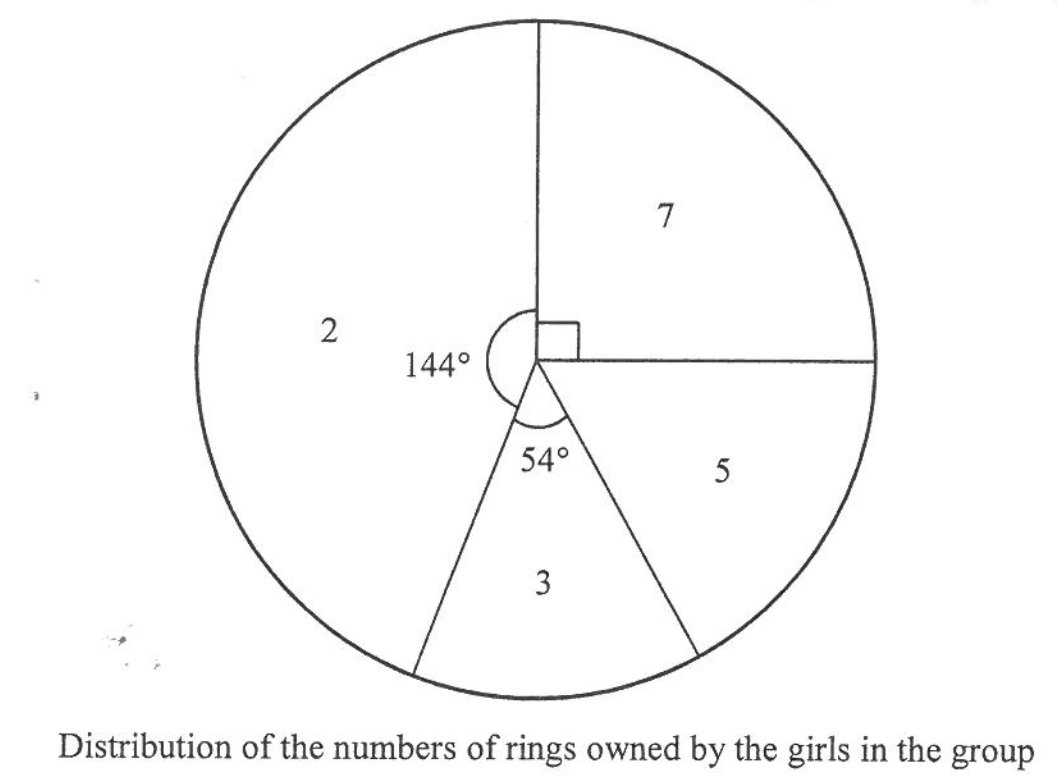
\includegraphics[width = .3\linewidth]{2019Figure1.00}
	\end{figure}
	\begin{enumerate}
		\item[(a)] Write down the mode of the distribution.
		\item[(b)] Find the mean of the distribution.
		\item[(c)] If a girl is randomly selected from the group, find the probability that the selected girl owns more than 3 rings.
	\end{enumerate}
	(5 marks)
	
	\item \textbf{HKDSE MATH CORE 2019 Past Paper I Q9}\\
	The sum of the volumes of two spheres is $324\pi$ cm3. The radius of the larger sphere is equal to the diameter of the smaller sphere. Express, in terms of $\pi$,
	\begin{enumerate}
		\item[(a)] The volume of the larger sphere;
		\item[(b)] The sum of the surface areas of the two spheres.
	\end{enumerate}
	(5 marks)

	\item \textbf{HKDSE MATH CORE 2019 Past Paper I Q10}\\
	It is given that $h(x)$ is partly constant and partly varies as $x$. Suppose that $h(-2) = -96$ and $h(5) = 72$.
	\begin{enumerate}
		\item[(a)] Find $h(x)$. \\(3 marks)
		\item[(b)] Solve the equation $h(x) = 3x^2$. \\(2 marks)
	\end{enumerate}

	\item \textbf{HKDSE MATH CORE 2019 Past Paper I Q11}\\
	Let $p(X)$ be a cubic polynomial. When $p(x)$ is divided by $x - 1$, the remainder is 50. When $p(X)$ is divided by $x + 2$, the remainder is $-52$. It is given that $p(x)$ is divisible by $2x^2 + 9x + 14$.
	\begin{enumerate}
		\item[(a)] Find the quotient when $p(X)$ is divided by $2x^2 + 9x + 14$. \\(3 marks)
		\item[(b)] How many rational roots does the equation   have? Explain your answer. \\(3 marks)
	\end{enumerate}

	\item \textbf{HKDSE MATH CORE 2019 Past Paper I Q12}\\
	The stem-and-leaf diagram below shows the distribution of the results (in seconds) of some boys in a 400 m race.
	\begin{table}[htbp]
		\centering
		\begin{tabular}{r|l@{\hspace{4 pt}}l@{\hspace{4 pt}}l@{\hspace{4 pt}}l@{\hspace{4 pt}}}
		   Stem (tens) & Leaf (units)     \\
			\hline
			5     & $a$\\    
			6     & 0 0 3 $c$ $c$ 8 9 9 9\\    
			7     & 0 1 1 1 2 2 5 6 9\\    
			8     & $b$\\    
		\end{tabular}
	\end{table}
	It is given that the inter-quartile range of the distribution is 8 seconds.	
	\begin{enumerate}
		\item[(a)] Find $c$. \\(2 marks)
		\item[(b)] It is given that the range of the distribution exceeds 34 seconds and the mean of the distribution is 69 seconds. Find
		\begin{enumerate}
			\item[(i)] $a$ and $b$,
			\item[(ii)] the least possible standard deviation of the distribution.
		\end{enumerate}
		(6 marks)
	\end{enumerate}

	\item \textbf{HKDSE MATH CORE 2019 Past Paper I Q13}\\
	In Figure 1, $O$ is the centre of circle $ABCDE$. $AC$ is a diameter of the circle. $BD$ and $OC$ intersect at the point $F$. It is given that $\angle AED = 115^\circ$.
	\begin{enumerate}
		\item[(a)] Find $\angle CBF$. \\(3 marks)
		\item[(b)] Suppose that $BC//OD$ and $OB = 18$ cm. Is the perimeter of the sector $OBC$ less than 60 cm? Explain your answer. \\(5 marks)
	\end{enumerate}

	\item \textbf{HKDSE MATH CORE 2019 Past Paper I Q14}\\
	In Figure 2, $ABCD$ is a square. It is given that $E$ is a point lying on $AD$. $BD$ and $CE$ intersect at the point $F$. Let $G$ be a point such that $BG // EC$ and $CG // DB$.
	\begin{enumerate}
		\item [(a)] Prove that 
		\begin{enumerate}
			\item[(i)] $\triangle BCG \cong \triangle CBF$,
			\item[(ii)] $\triangle BCF \sim \triangle DEF$.
		\end{enumerate}
		(4 marks)
		\item[(b)] Suppose that $\angle BCF = \angle BGC$.
		\begin{enumerate}
			\item [(i)] Let $BC = l$. Express $DF$ in terms of $l$.
			\item[(ii)] Someone claims that $AE > DF$. Do you agree? Explain your answer.
		\end{enumerate}
		(4 marks)
	\end{enumerate}

	\item \textbf{HKDSE MATH CORE 2019 Past Paper I Q15}\\
	There are 21 boys and 11 girls in a class. If 5 students are selected from the class to form a committee consisting of at least 1 boy, how many different committees can be formed?	 \\(3 marks)

	\item \textbf{HKDSE MATH CORE 2019 Past Paper I Q16}\\
	Let $\alpha$ and $\beta$ be real numbers such that $\left\{\begin{matrix}
		\beta  =  5\alpha  -  18 \\
		\beta = \alpha^2 - 13\alpha + 63\\
		\end{matrix}\right.$ .
	\begin{enumerate}
		\item[(a)] Find $\alpha$ and $\beta$. \\(2 marks)
		\item[(b)] The 1st term and the 2nd term of an arithmetic sequence are $\log{\alpha}$ and $\log{\beta}$ respectively. Find the least value of $n$ such that the sum of the first $n$ terms of the sequence is greater than 888. \\(4 mark)
	\end{enumerate}

	\item \textbf{HKDSE MATH CORE 2019 Past Paper I Q17}
	\begin{enumerate}
		\item[(a)] Let $a$ and $p$ be the area and the perimeter of $\triangle CDE$ respectively. Denote the radius of the inscribed circle of $\triangle CDE$ by $r$. Prove that $pr = 2a$. \\(2 marks)
		\item[(b)] The coordinates of the points $H$ and $K$ are $(9, 12)$ and $(14, 0)$ respectively. Let $P$ be a moving point in the rectangular coordinate plane such that the perpendicular distance from $P$ to $OH$ is equal to the perpendicular distance from $P$ to $HK$, where $O$ is the origin. Denote the locus of $P$ by $\Gamma$.
		\begin{enumerate}
			\item[(i)] Describe the geometric relationship between $\Gamma$ and $\triangle OHK$.
			\item[(ii)] Using (a), find the equation of $\Gamma$.
		\end{enumerate}
		(5 marks)
	\end{enumerate}

	\item \textbf{HKDSE MATH CORE 2019 Past Paper I Q18}\\
	Figure 3 shows a tetrahedron $ABCD$. Let $P$ be a point lying on $AD$ such that $BP$ is perpendicular to $AD$. A craftsman finds that $AC = AD = CD = 13$ cm, $BC = 8$ cm, $BD = 12$ cm and $\angle ABD = 72^\circ$.
	\begin{figure}[H]
		\centering
		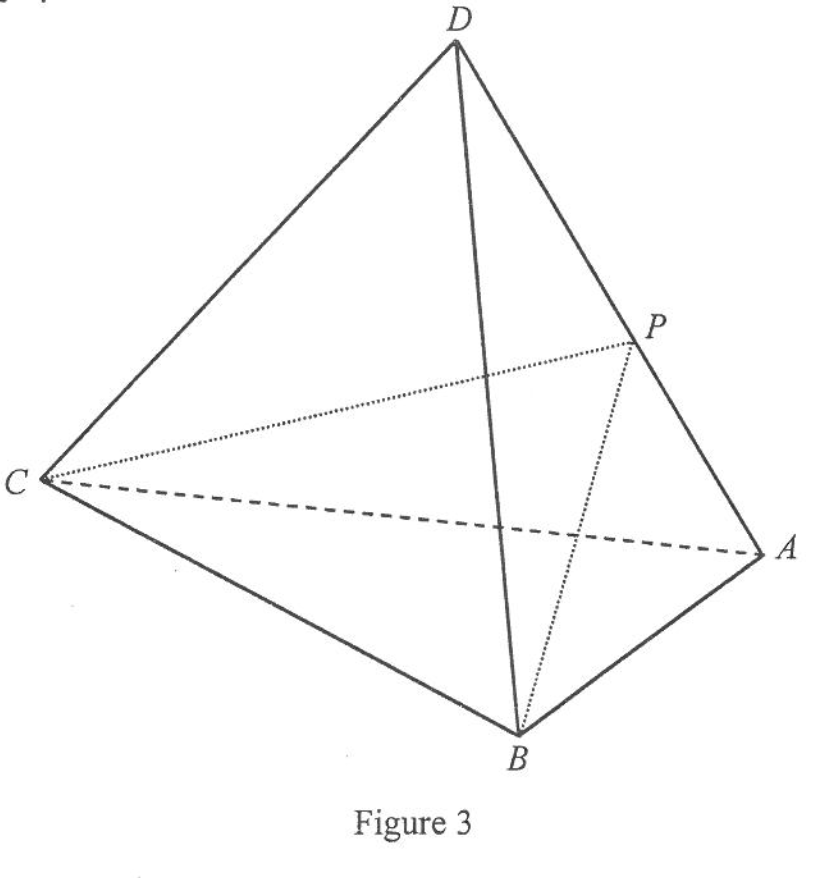
\includegraphics[width = .3\linewidth]{2019Figure1.3}
	\end{figure}
	\begin{enumerate}
		\item[(a)] Find
		\begin{enumerate}
			\item[(i)] $\angle BAD$,
			\item[(ii)] $CP$.
		\end{enumerate}
		(5 marks)
		\item[(b)] TThe craftsman claims that $\angle BPC$ is the angle between the face $ABD$ and the face $ACD$. Is the claim correct? Explain your answer. \\(2 marks)
	\end{enumerate}

	\item \textbf{HKDSE MATH CORE 2019 Past Paper I Q19}\\
	Let $f(x) = \dfrac{1}{1 + k}(x^2 + (6k - 2)x + (9k + 25))$, where $k$ is a positive constant. Denote the point $(4, 33)$ by $F$.
	\begin{enumerate}
		\item[(a)] Prove that the graph of $y = f(x)$ passes through $F$. \\(1 mark)
		\item[(b)] The graph of $y = g(x)$ is obtained by reflecting the graph of $y = f(x)$ with respect to the $y$-axis and then translating the resulting graph upwards by 4 units. Let $U$ be the vertex of the graph of $y = g(x)$. Denote the origin by $O$.
		\begin{enumerate}
			\item[(i)] Using the method of completing the square, express the coordinates of $U$ in terms of $k$.
			\item[(ii)] Find $k$ such that the area of the circle passing through $F$, $O$ and $U$ is the least.
			\item[(iii)] For any positive constant $k$, the graph of $y = g(x)$ passes through the same point $G$. Let $V$ be the vertex of the graph of $y = g(x)$ such that the area of the circle passing through $F$, $O$ and $V$ is the least. Are $F$, $G$, $O$ and $V$ concyclic? Explain your answer.
		\end{enumerate}
		(11 marks)
	\end{enumerate}


\end{enumerate}
\end{document}